\documentclass{article}
\usepackage{float}
\usepackage{geometry}
\usepackage{graphicx}
\usepackage[utf8]{inputenc}
\usepackage{hyperref}
\usepackage{cite}
\geometry{margin = 0.8in}

\title{10-701 Project Proposal}
\author{Roger Jin, Alexander Yu}
\date{}

\begin{document}
\maketitle

\section{Introduction and Problem Setup}
A current topic of interest in Computer Vision is grounding, that is, linking image representations to the semantic content found in other modalities such as language. While object classification can be seen as a rudimentary form of grounding, vis-a-vis linking images to a set of known text labels, a more challenging problem is caption generation from images. The aim of this project is to use existing methods that generate representations from image and text to build a network that can jointly learn those representations. To that end, we will assess the impact of two variables on performance: 1) existing methods of generating representations and 2) architectures for the image to text model.
 
\section{Background and Literature}
The Contrastive Language Image Pretraining (CLIP) model is the primary inspiration for this project and treats caption generation as a zero-shot classification task \cite{radford2021learning}. CLIP jointly trains an image encoder and text encoder with text-image pairs. For each text-image pair, a classifier trains to associate the latent representation of the text with the latent representation of the image (hence its "contrastive" nature). At test time, CLIP is provided with an image and a sentence fragment to complete. For example:
\begin{center}
    "A photo of a \underline{\hspace{0.75in}}, a type of food"
\end{center}
Leveraging context from the incomplete sentence and information from the image allows CLIP to achieve roughly 40\% zero-shot classification accuracy on the ImageNet dataset. While generation of captions from scratch is not CLIP's intended purpose, captions can be generated by passing CLIP's previous output sentence as the input fragment to a subsequent iteration. 

\section{Methods/Model}
While CLIP treats the association between text and images as a classification task, we propose a model which associates text and images through regression. The steps to constructing this proposed model are as follows:
\begin{enumerate}
    \item Train or find a pre-trained image autoencoder. Convolutional Res-Net Autoencoders are a promising option.
    \item Train or find a pre-trained text autoencoder. Tranformers are a promising option \cite{9373350}.
    \item Train a regression model (denoted the "Transform Network") which transforms the image's latent representation to the text's latent representation. While training the Transform Network, the text and image autoencoders' weights are frozen.
\end{enumerate}
 This allows for end-to-end caption generation, whereas CLIP is only able to fill in missing phrases in sentences from a predefined set of classes. Furthermore, our approach does not require that the image and text autoencoders be jointly trained; each autoencoder may be pre-trained or trained separately and the Transform Network should be trainable on a smaller set of text-image pairs. However, our proposed model loses CLIP's zero-shot capabilities. Figure 1 shows a graphical representation of the model.
\begin{figure}[H]
    \centering
    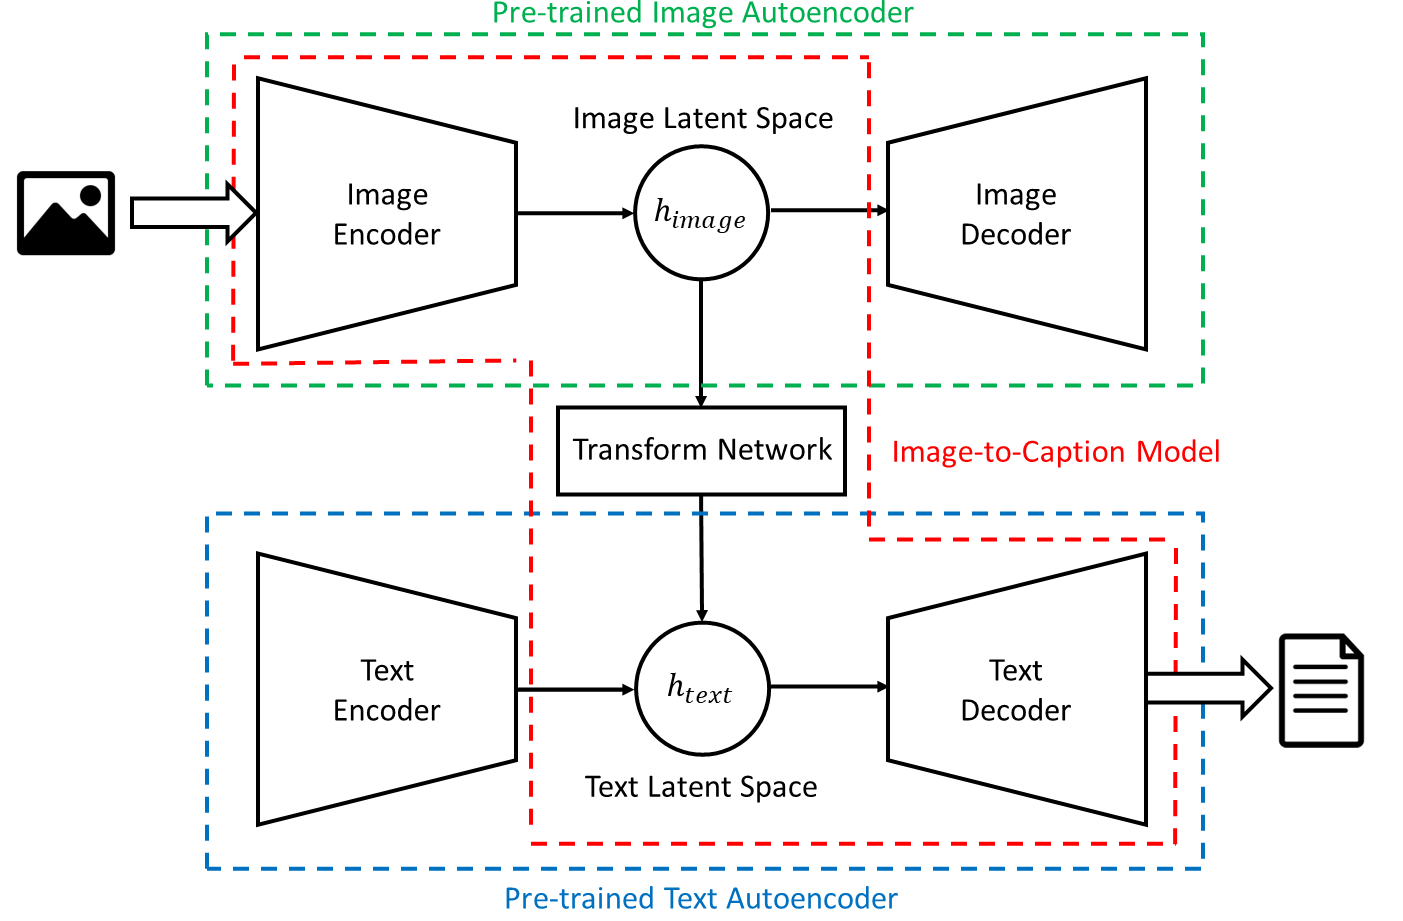
\includegraphics[width=0.8\textwidth,keepaspectratio]{Network Overview.png}
    \caption{Overview of the proposed image to caption network. The image decoder and text encoder are used for training only and are not used at test time. Gradients will \textit{not} propagate through the Transform Network into the image encoder.}
\end{figure}

\section{Data}
To train the image to text model, we will use the Common Objects in Context (COCO) dataset which contains roughly 200,000 annotated images with 5 captions per image \cite{DBLP:journals/corr/LinMBHPRDZ14}. All images contain at least one of 91 object types, each of which can be easily identified in an image by a human. Because the objects in its constituent images are readily identifiable, COCO is a useful benchmark in assessing the baseline capabilities of our text to image model; if we cannot even learn captions for common objects, it may be harder yet to learn captions for uncommon ones. \\

\section{Evaluation Criteria}
We will evaluate the quality of generated captions both quantitatively and qualitatively. In terms of quantitative evaluation, we will compare the learned text representation to the learned text representation of each of the ground truth captions on a holdout set of COCO. In terms of qualitative evaluation, we will generate a separate small test set containing objects not found in the COCO dataset and determine whether the generated captions are accurate. Since caption generation is, at its core, an exercise in grounding, testing on unseen examples is needed to interrogate the generality of the semantic content the model can link to images. For both the qualitative and quantitative evaluations, we will compare against existing pre-trained models such as CLIP as baselines. 

\bibliographystyle{ieeetr}
{\footnotesize
\bibliography{references.bib}}
\end{document}
